\documentclass[12pt,a4paper]{report}

% English
\usepackage[english]{babel} % English language setting
\usepackage[utf8]{inputenc} % Unicode text
\usepackage[T1]{fontenc} % German 'Umlaute'
\usepackage{textcomp} % Euro
\usepackage[hyphens]{url}
\usepackage{amssymb} % Symbols
\usepackage{emptypage} % Empty pages are now actually empty

% Fonts, with all the options
\usepackage{mathpazo}
\usepackage[scaled=.95]{helvet}
\usepackage{courier}
\usepackage{microtype}

% Images and listings
\usepackage{graphicx} % images
\usepackage{subfig} % sub-figures
\usepackage{wrapfig} % wrapping figures
\usepackage{listings} % better source code listings
\usepackage{enumitem}
\graphicspath{ {figures/} }

% Source code
\usepackage{float}
\newfloat{listing}{htbp}{scl}[chapter]
\floatname{listing}{Listing}
\usepackage{packages/coding/golang/lang} % import this package after listings
\usepackage{packages/coding/protobuf/lang}  % include language definition for protobuf
\usepackage{packages/coding/protobuf/style} % include custom style for protobuf declarations.
\lstset{
    basicstyle=\scriptsize\ttfamily,
    columns=[l]flexible,
    mathescape=true,
    showstringspaces=false,
    numbers=left,
    numberstyle=\tiny,
    frame=none,
    keywordstyle=\color{red},
    stringstyle=\color{blue},
    showstringspaces=false,
    tabsize=4,
    xleftmargin=\leftmargin,
    language=Golang
}

% Page layout
\usepackage[paper=a4paper,width=14cm,left=35mm,height=22cm]{geometry}
\usepackage{setspace}
\usepackage[htt]{hyphenat}
\usepackage{sectsty}
\linespread{1.5}
\subsubsectionfont{\large}

% Page markers
\newcommand{\phv}{\fontfamily{phv}\fontseries{m}\fontsize{10}{12}\selectfont}
\usepackage{fancyhdr} % nicer header and footer
\pagestyle{fancy}
\renewcommand{\chaptermark}[1]{\markboth{#1}{}}
\fancyhead[L]{\phv \nouppercase{\leftmark}}
\fancyhead[R]{\phv \thepage}
% rather not use anything for the footer
\fancyfoot[C]{\ } % no page count in the bottom
%\fancyfoot[R]{\textsf{\small Media Management}}

% Share the sources
\usepackage{bibtopic}

% Logo of the university
\usepackage{packages/hsrmlogo}

% Special packages
\usepackage{epigraph}
\setlength{\epigraphrule}{0pt} % no divider
\usepackage{csquotes}

% Some extra styles
\usepackage{soul}
\newcommand*\strikethrough{\st}

% Hyperlink everything
\usepackage{hyperref}
\hypersetup{
    bookmarks=true,
    colorlinks=true,
    linkcolor=black,
    citecolor=black,
    filecolor=black,
    urlcolor=black,
}
\urlstyle{same}

% Wikipedia-style "citation needed" macro
\newcommand{\cn}[1][]{\textsuperscript{\color{red} ~[citation needed]~}}

% Code markup
\newcommand{\code}[1]{\texttt{#1}}


\newcommand{\studyprogramme}{Media Management}
\newcommand{\degreetype}{Bachelor of Arts}
\newcommand{\thesistitle}{
The system and software architecture of back-end applications for the short-term rental of electric scooters
}
\newcommand{\thesissubtitle}{
Analysis of an existing legacy solution and evaluation of its extensibility
}
\newcommand{\thesisauthor}{Jakob Löhnertz}
\newcommand{\thesisdate}{23. Juli 2018}
\newcommand{\thesislocation}{Wiesbaden}
\newcommand{\firstmarker}{Prof.\ Dr.\ Johannes Luderschmidt}
\newcommand{\secondmarker}{Merle Hiort}

\begin{document}

\begin{titlepage}
  \begin{center}
    \hsrmlogo[1]
    \parbox[t]{8cm}{
      Hochschule \textbf{RheinMain}\\
      Fachbereich Design Informatik Medien\\
      Studiengang \studyprogramme}
    \\[1.5cm]
    {\LARGE Abschlussarbeit} \\[0.5cm]
    {\begin{spacing}{1} \large zur Erlangung des akademischen Grades \\[5mm] \end{spacing}}
    {\begin{spacing}{1} \large \degreetype \\[1cm] \end{spacing}}
    \rule{\textwidth}{1pt} \\[0.5cm]
    {\begin{spacing}{1.15} \huge \bfseries \thesistitle \\ \end{spacing}}
    {\begin{spacing}{1.15} \bfseries \thesissubtitle \\[0.60cm] \end{spacing}}
    \rule{\textwidth}{1pt}
    \\[1.5cm]
    \begin{tabular}{ll}
      Vorgelegt von & \thesisauthor \\
      am & \thesisdate \\
      Referent & \firstmarker \\
      Korreferent & \secondmarker
    \end{tabular}
  \end{center}
\end{titlepage}
\cleardoublepage

% Erklärung gemäß den Allgemeinen Bestimmungen für Prüfungsordnungen
\thispagestyle{empty}
\section*{Erklärung gemäß ABPO}
Ich erkläre hiermit, dass ich
\begin{itemize}
\item die vorliegende Abschlussarbeit selbstständig angefertigt,
\item keine anderen als die angegebenen Quellen benutzt,
\item die wörtlich oder dem Inhalt nach aus fremden Arbeiten entnommenen
  Stellen, bildlichen Darstellungen und dergleichen als solche genau
  kenntlich gemacht und
\item keine unerlaubte fremde Hilfe in Anspruch genommen habe.
\end{itemize}

\vspace{6em}
\noindent\begin{tabular}{p{0.37\textwidth}p{0.56\textwidth}}
\thesislocation, \thesisdate  & \rule{0.56\textwidth}{0.5pt}\\
              & \makebox[1cm]{\ } \thesisauthor
\end{tabular}

\vfill

\cleardoublepage



\begin{abstract}

The abstract will be added at this place towards the end of the thesis.

\end{abstract}


\tableofcontents



\chapter{Problems and research question} \label{chap:intro}

\epigraphhead[55]{\epigraph{Beauty is more important in computing than anywhere else
in technology because software is so complicated. Beauty is the ultimate defense against complexity.}
{\textit{David Gelernter}}}


The definition of the word \emph{scooter} is fairly vague.
Some describe it as a small vehicle with a handlebar and a platform to stand on,
the kind traditionally children were riding.
However, this paper looks at the \emph{motorcycle-esque type} of a scooter, and in
particular the electric version of it.

Many pain points of internal combustion engines vanish with the switch to their electric
counterparts. The maintenance of the mechanical system of the whole vehicle becomes easier.
There are less moving parts which makes for less errors.
On the downside, the exchange of the fuel causes the most problems with electric engines.
Of course they utilize batteries instead of fossil fuels as their impetus.
Although the invention of the battery is older than that of the
internal combustion engine\cn, the technology is still not perfected and sees new
advancements every year. Alas, it also combats many challenges in terms of
safety, cost, capacity, weight, recycling, speed of recharging and longevity.

For the provider, the handling of a short-term rental service
only becomes feasible with the automation of as many processes as possible.
This requires a back-end application ideally paired with a front-end.
Most of the time, ongoing human resource costs make up the biggest percentage
in the expenses of any business.\cn Thus, this demands for less human workforce
as part of the processes of a rental service.
Meanwhile, the upfront expenditures for the software development of
an application are still vast but in the long run, the running expenses are less.
The only cost driver afterwards is the maintenance of the created software.
As a consequence, the question should be how to mitigate the maintenance costs
of a software product. The main aspect is a proper application of
software engineering which is defined as:
\begin{displayquote}
\emph{"The application of a systematic, disciplined, quantifiable approach to the
development, operation, and maintenance of software."}~\cite{se-ieee}
\end{displayquote}
As a consequence, section \ref{sect:software-development-process} exhibits
said approach in great detail.

Furthermore, the fact that the scooters are always connected to the internet
as well as the nature of current batteries desire a reactive and faultless application.

Finally, the corporate partner of this thesis, which is discussed in detail
in section \ref{sect:kumpan}, is already in possession of a solution which is not fully featured yet.
Therefore, the subject of extending an existing back-end application with missing features is also targeted.

In conclusion, this leads into the research question of this bachelor thesis:\\
\emph{Which functional modules are necessary for the implementation of a back-end application
for the short-term rental of electric scooters and which considerations need to be made
to integrate additional functionality into an existing legacy software solution for that purpose?}



\chapter{Fundamentals} \label{chap:fundamentals}

\epigraphhead[55]{\epigraph{The danger in the sequence [waterfall approach]
is that the project moves from being grand to being grandiose,
and exceeds our human intellectual capabilities for management and control.}
{\textit{Harlan D. Mills}}}


\section{The market for the rental of electric scooters} \label{sect:electric-scooter-market}

The market for the short-term rental of motor vehicles in Germany
is currently growing rapidly~\cite{bundesverband-carsharing-statistics}.
The situation on the market is no different for medium and long-term rentals~\cite{sparkasse-kfz-vermietung}.
However, this sector is dominated by cutthroat competition.
It has been dictated by large corporations such as \textit{Sixt}, \textit{Hertz},
\textit{Avis} and \textit{Europcar} for years~\cite{sparkasse-kfz-vermietung}.
Although smaller providers exist, this market has become an oligopoly and
the barriers for a market entry are high for new types of providers.

In contrast, the market for short-term rental, also known as \textit{car sharing} for cars,
is a comparatively young market. It has only existed in Europe in its breadth
since the late 1980s~\cite{history-of-carsharing} and in its current form
only since the advent of the smartphone, since many offers require the use of a mobile app.
For this reason the market for short-term rentals and thus its saturation is significantly lower.
According to the \textit{Bundesverband CarSharing e.V.}, the current total number of cars
in the car sharing sector in Germany is about 17,200. In contrast, almost 10\% of all
new vehicle registrations in Germany in 2015 were attributable to traditional
car rental companies such as the above~\cite{sparkasse-kfz-vermietung}.
This represents an increase of 339,000 vehicles, in similar fashion every year.
By contrast, the share of vehicles with electric drive is again lower at
just under 10\% of the total number of car sharing vehicles.
Electric scooters do not even appear in the statistics of the
\textit{Bundesverband CarSharing e.V.}~\cite{bundesverband-carsharing-statistics}.

However, the market in other nations has already experienced strong growth;
one example is the Chinese market. Around 20 million electric scooters were sold
there in 2016 alone~\cite{heise-electric-scooters}. Market value forecasts are also promising.
Last year, the US company \textit{P\&S Market Research} predicted an annual growth of
just under 7\% in the market for motorized two-wheeled vehicles with
electric drive until 2025~\cite{pands-electric-scooters}.
The future of the market is promising, as more and more nations around the world
are deciding on a ban on vehicles with internal combustion engines for the
foreseeable future~\cite{faz-combustion-engine-ban}.

Nevertheless, there are already working business models in European cities
which can yield additional information.
According to the \textit{Global Scootersharing Market Report 2017} by the
\textit{Innovation Centre for Mobility and Societal Change (InnoZ) GmbH},
the short-term rental of scooters in general consist 92\% of scooters with
electric drive. Additionally, 95\% are so-called \textit{free-floating systems},
meaning that each customer can drop off the scooters wherever they want, regardless
of their current location as long as it is within the available area of the offering operator.
However, this system also implies that the operating organization needs personnel
and equipment to relocate scooters that were discarded in areas with low demand.
Finally, three main models do exist for billing the customers~\cn.
Namely, these are billing per minute, billing per kilometer, or a fixed rate for a whole ride.


\subsection{German electric scooter manufacturer \textit{Kumpan}} \label{sect:kumpan}

The thesis loosely focuses on the business of German electric scooter manufacturer \textit{Kumpan}.
The company was established in 2009. For their product, they concentrated on three main aspects:
an exterior design ready for the European market, build quality and sufficient cruising radius.
They finished building their first electric scooter in 2010 and are thriving for good products ever since.
The price of their electric scooters is still rather high. Owing to that circumstance,
they came up with smaller, cheaper models as well as a completely different approach.

Instead of traditional retail sales they started developing the idea of a
short-term rental service for their scooters. And from many angles it makes sense:
As seen in the last section, the market for the short-term rental of electric scooters
especially in Germany is still minuscule compared to e.g. car or bike sharing.
Meanwhile, the costs for buying an electric scooter are still relatively high.
Additionally, many people will not need such a vehicle for the whole day and would benefit
from more flexibility. Lastly, parking spots are also a scarcity in inner cities.
Therefore, \textit{Kumpan} plans to enter the market of short-term electric scooter rentals
in the near future.

There are still many aspects to be discussed and determined but one of them
is already set and can be seen as a necessity regardless of the final implementation:
A server back-end application as well as its infrastructure.
\textit{Kumpan} purchased an existing software solution to achieve this.
Beforehand, it was already known though that the software is not feature-complete
for their usage. Thence, it is already planned to extend the software with the missing
features.


\section{Components of a modern software product} \label{sect:frontend/backend}

The main aspect of success for such a system is the \textit{magic} behind the scenes
that no customer sees. People just see the electric scooter as the product and
want to be able to ride one on demand by just pushing a button.
The ease of use for the customers and their satisfaction are the main facets
to be considered by the provider of such a service.

Oftentimes this, as virtually all the short-rental services on the market~\cn,
involves two foundational web-based components --- a front-end and a back-end\cn.
On the one hand, the front-end provides the user interface of the product, the façade of the whole.
It is the component the customer interacts with but more importantly it will be
what the users identify the product with.
On the other hand, the back-end is the brain of the software product.
It provides endpoints for the front-end to use and consume. The back-end dictates
what the front-end will do. Meanwhile, it does not determine what it will look like.
If the front-end is unusable the back-end will never be able to fix that as the
front-end becomes the mental representation of the whole product for the customers.
If the back-end behaves sluggish or is prone to errors, the front-end will not be able to save much
by the same token. In the end, both form a synergy with each other.

This thesis will shed light on the back-end of such an application.
It will focus on the system and software architecture of it.
This includes the functionalities that are mandatory and the question on
how the product might come together; from ideas and drafts to written source code.


\subsection{Necessity of a thorough back-end application}

A look at existing car sharing offers depicts that automating the rental process
is necessary. There are three main aspects that become easier to achieve for the
provider if they choose to automate their system.\\
Firstly, as already mentioned in the first chapter,
the costs are a lot lower whenever less human resources are involved.
Additionally, the speed of execution of a rental request by a customer gets better
with a performant back-end application.
Finally, a modern software solution attracts more customers as the ease of use
is expected to be better. Furthermore, the entrance barrier to try a rental service
gets lower. Nowadays, customers, especially younger ones, are used to web-based
or mobile app-based software and are a lot more likely to try out such an offer.~\cn
Although, the users are never in contact with the back-end, it is absolutely
crucial for the success of the whole application as the front-end just displays
the information in a presentable way while not performing any serious
business logic most of the time.


\section{Approaching the development of software} \label{sect:software-development-process}

From a very fundamental standpoint, software development consists of two distinct phases.
The planning and analysis phase which leads into the programming phase~\cite{royce-large-systems}.
Upon further investigation, there are more steps before, in between and after these two essential ones.
In his influential 1970 paper \textit{"Managing the Development of Large Software Systems"},
American computer scientist Winston W. Royce discusses his idea of a satisfactory
software development process. His paper is often mistakenly cited as the starting point
of the \textit{waterfall model} whereas Royce indeed starts his paper with such an approach but quickly
depicts the shortcomings of that model~\cite{royce-large-systems, larman-iid-history}.
The waterfall model describes the idea that a software development process should consist of
the stages shown in figure \ref{fig:waterfall-model}.
\begin{figure}[htbp]
\centering
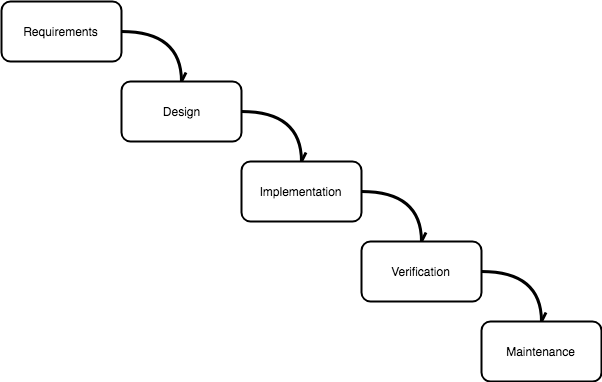
\includegraphics[width=.60\textwidth]{waterfall-model}
\caption{The essential stages of the waterfall model}
\label{fig:waterfall-model}
\end{figure}
The main point of it is that the steps are conducted sequentially;
no step should begin before the current one has been finished~\cite{boehm-spiral}.
This idea has one big flaw: the \textit{Verification} phase being nearly at the end.
Only after the whole software product is finished, an evaluation by internal testing personnel or
the client can be carried out~\cite{royce-large-systems}.
It is likely that at least some changes to the implementation will be necessary after the \textit{Verification}.
Additionally, clients may not know the exact requirements at the very beginning
of the software development process~\cite{parnas-rational-design-process}.
It is also possible that a major fault is only discovered in that second last stage ---
the negative repercussions could be massive.
\begin{displayquote}
\emph{"Either the requirements must be modified, or a substantial change
in the design is required. In effect the development process has returned to
the origin and one can expect up to a 100-percent overrun
in schedule and/or costs."}~\cite{royce-large-systems}
\end{displayquote}
Nevertheless, the idea Royce describes is what made his paper as influential.
The steps that are required to get from an idea to a finished product nearly always
stay the same. The ones from figure \ref{fig:waterfall-model} are still applicable to
many newer concepts of a software development process.

Nowadays, software developers and project managers are mostly utilizing any model that
can be subsumed under the loose term \textit{agile}.
In summary, as the term already depicts, this theory is geared towards
the idea that the software development process should not be as rigid and constrained.
Therefore, it stands in stark contrast to the demonstrated waterfall model.
The term does not describe an explicit concept but rather an idea ---
there are dozens of implementations of agile software development~\cite{martin-agile-practices}.
Regardless of the implementation, most often agile approaches are based around
the idea of \textit{Iterative and Incremental Development (IID)}~\cite{larman-iid-history}.
\begin{displayquote}
\emph{"Software development should be done incrementally, in stages with
continuous user participation and replanning and
with design-to-cost programming within each stage."}~\cite{mills-iid}
\end{displayquote}
Instead of implementing the whole software within all the sequential steps
of the waterfall model, the product is being developed in increments.
Following some initial analyzing and planning, the first iteration begins.
After the end of one iteration of all the steps shown, apart from the \textit{Maintenance},
the next increment is getting projected and eventually executed as shown in figure \ref{fig:idd-model}.
\begin{figure}[htbp]
\centering
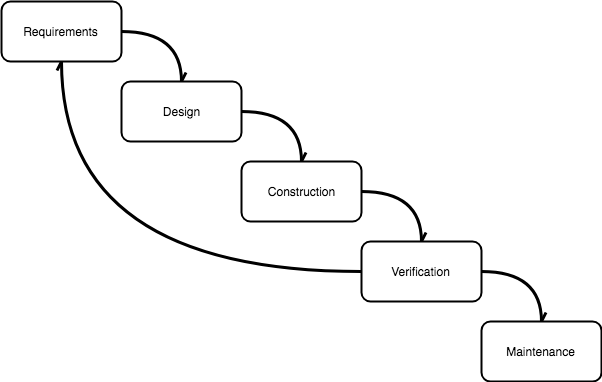
\includegraphics[width=.60\textwidth]{iterative-and-incremental-model}
\caption{A revised, iterative version of the waterfall model e.g. IID}
\label{fig:idd-model}
\end{figure}\newline
To conclude, the stages Royce exhibited in 1970 are still applicable nowadays.
In some form or another, those are mandatory for implementing any software
and became therefore known as the \textit{software development life cycle}.~\cite{se-ieee}
This fact is corroborated by the IEEE's
\textit{Guide to the Software Engineering Body of Knowledge (SWEBOK)}
which is also recognized by the ISO~\cite{swebok}.
This document defines \textit{"knowledge areas"} which match the depicted stages.\\
Consequently, the portrayed stages are discussed in greater detail in the following subsections,
while excluding the last two ones as they will not be part of the
\textit{\nameref{chap:analysis}} chapter.
Moreover, these explanations do not follow an incremental approach
or a sequential one --- the point of view is generalized.


\subsection{Requirements} \label{subsect:requirements}

The \textit{SWEBOK} by IEEE defines \textit{Software Requirements} as:
\begin{displayquote}
\emph{"The Software Requirements knowledge area (KA) is concerned with
the elicitation, analysis, specification, and validation of software requirements
as well as the management of requirements during the whole
life cycle of the software product."}~\cite{swebok}
\end{displayquote}
Generally speaking, two types of requirements do exist --- functional and non-functional ones.
Functional requirements are definitive features of the software whereas non-functional
requirements are describing aspects of the software like performance, security,
user-friendliness and so forth~\cite{sommerville-se}.\\
Furthermore, requirements should be quantifiable; specific key figures should be established
rather than broad statements like \textit{"overall great performance"}.\\
Finally, after specifying the gathered requirements a validation of them should be conducted.
This validation process is not part of this subsection though.


\subsubsection{Elicitation}
Requirements elicitation describes the process of gathering the requirements.
Many stakeholders are part of this process e.g. the customer, software engineers,
available users or a market analysis and the management of the organization conducting
the development.
During the elicitation, proper communication between these parties is the most important
concern. Additionally, the stakeholders should always seek for a set of
requirements that is still extensible later on~\cite{swebok}.

\paragraph{Sources}
The goal or objective of the software should be known and can be used to
shape the overall requirements of the finished product.
Moreover, the engineers and developers should utilize their knowledge especially
toward the customer who usually does not know much about software development.
Doing this, many early requirements by the customer can be rationalized to allow
them to still be included albeit in a reasonable form.
Additionally, all the stakeholders should seek for a balance between them in
terms of their standpoints and requests.\\
Finally, three sources remain that are derived from the organization and its sector.
Namely, these are the organizational, operational, and business environments~\cite{swebok}.

\subparagraph{Organizational environment}
The employees of the organization are oftentimes the ones who use the software
directly or indirectly. Thus, the developed software should fit into the existing
organizational businesses processes. In case a disruption of any business process
is expected due to the new software, this affair should be discussed with the
employees of the organization.

\subparagraph{Operational environment}
The environment where the software will later be run is also important for the
aggregation of requirements. If a certain performance is mandatory for the use case
of the software, this should be formed into a concrete requirement.

\subparagraph{Business environment}
Commonly, the business of the organization dictates certain requirements like
payments. For example, for paid services a preeminent requirement is that
no customer should be able to circumvent the payment.


\paragraph{Techniques}
After the sources of the requirements are clarified, certain techniques can be
applied to actually gather them~\cite{sommerville-se, swebok}.\\
Interviews are seen as the most basic form of requirements elicitation;
during these the stakeholders are getting interviewed to garner possible requirements.
Similarly, meetings with all the stakeholders can be conducted to discuss the requirements.
The advantage of this approach is that every stakeholder brings other considerations and
different knowledge into the meeting which allows for better discussions.
Furthermore, prototypes can be created to collect requirements early on while already
receiving feedback for existing ones. Moreover, scenarios and observations can be
conducted. A scenario looks at the use case of the software from the standpoint
of the software engineers while an observation focuses on the perspective of the
users. With the latter technique, it is often possible to discover requirements
that were to minuscule to be mentioned by the other stakeholders or even by the users themselves.


\subsubsection{Analysis}

The analysis and later specification of the requirements begins with the classification
of them and leads into some form of modeling.

\paragraph{Classification}
As already mentioned, the most basic form of classifying requirements is to group
them into functional and non-functional ones. Moreover, it should be discerned
wether a requirement is high-level or low-level in terms of its implementation.
Additionally, the scope of the requirement can be a deciding factor.
If a requirement has major implications on the whole software, it should be classified
differently than a specific but small feature. Similarly, the stakeholders should
estimate how stable a requirement is; if it is likely to change, it should not
play an integral role in the whole system.
Finally, it should be determined how high or low the priority of each requirement is.
This can lead to a more focused design and implementation with regard to achieving
a \textit{minimal viable product (MVP)} sooner than later during
the development process~\cite{swebok, sommerville-se}.

\paragraph{Specification}
After the requirements are classified, they can be modeled into e.g.
a natural language specification or a diagram.
The \textit{SWEBOK} by IEEE mentions \textit{"use case diagrams, data flow models,
state models, goal-based models, user interactions,
object models, data models, and many others."}~\cite{swebok}
The \textit{Unified Modeling Language (UML)} offers good, standardized diagrams
to create these conceptual requirements models.
Moreover, Ian Sommerville states that natural language documents
are still the most widely used form of requirements specification as they are
\textit{expressive, intuitive, and universal}~\cite{sommerville-se}.


\subsection{Design} \label{subsect:design}

Software design is defined as: \textit{"the process of defining
the architecture, components, interfaces, and other characteristics
of a system or component"}~\cite{iso-se}.
The result of said process is the software architecture which describes the
components of the software as well as their interfaces~\cite{swebok}.
However, software architecture has two layers: the high-level design as well as
the low-level design which is about the more detailed
construction of single components~\cite{iso-sdlc}.
Usually, the functional requirements mentioned in the previous subsection dictate
what the low-level architecture will look like. In contrast, non-functional
requirements often determine the high-level architectural design of an application~\cite{bosch-sa}.
However, oftentimes a mixture of both will determine both aspects of the final software architecture.


\subsubsection{Design decisions}

As the word \textit{decision} depicts, \textit{Design decisions} are all about
answering questions regarding the software design. While contemplating about
the answer to each question, the software architecture increasingly emerges.
Additionally, if every decision is made, the architecture automatically gains
sophistication. Ian Sommerville states nine \textit{Design decisions} in his
standard work \textit{Software Engineering}~\cite{sommerville-se}.
For this thesis, four of them were picked to be substantive:
\begin{enumerate}
\item What architectural patterns or styles might be used?
\item What architectural organization is best for delivering the non-functional requirements of the system?
\item What will be the fundamental approach used to structure the system?
\item What strategy will be used to control the operation of the components in the system?
\end{enumerate}
Furthermore, the engineers should think about the following five non-functional characteristics:
\textit{Performance}, \textit{Security}, \textit{Safety}, \textit{Availability},
and \textit{Maintenance}~\cite{sommerville-se}. However, how exactly these are
regarded and achieved is not part of this subsection.


\subsubsection{Principles}

Regardless of the final software architecture, software design principles exist
that are shared and applied in some way by every software; the \textit{SWEBOK} by IEEE
mentions seven of them~\cite{swebok}: \textit{Abstraction}, \textit{Coupling and Cohesion},
\textit{Decomposition and Modularization}, \textit{Information Hiding},
\textit{Separation of Interface and Implementation},
\textit{Sufficiency and Completeness}, and \textit{Separation of Concerns}.
Ideally, if applied correctly, these principles greatly improve the structure
of any software which in return enhance other areas of the
software development process like maintenance. All of the mentioned
software design principles are discussed briefly in the following paragraphs.

\paragraph{Abstraction}
\textit{Abstraction} is about perspective; it tries to achieve that an object or
function only focuses on the information that is mandatory for the execution of
their task while not taking account of the full set of information.
For instance, a function that is used in two locations of an application
should be abstract enough to be used in a third one later on without
any modifications to it.

\paragraph{Coupling and Cohesion}
These two terms are describing how a component behaves in regard to the whole application.
\textit{Coupling} is a measure of the interdependence of a component whereas
\textit{Cohesion} describes how associated the elements of the components are~\cite{swebok}.
Consequently, this concept is therefore close to the aforementioned \textit{Abstraction}
since high \textit{Coupling} lowers the abstraction of a system and vice versa.

\paragraph{Decomposition and Modularization}
Software should be divided into components and even sub-components that each fulfill
an unique task while having concrete interfaces to interact with each other.
Oftentimes, the resulted components are called modules hence the term \textit{Modularization}.

\paragraph{Information Hiding}
From the outside of a component, the internals of its implementation should be hidden.
Thus, data should only be accessed via an interface which in return makes it irrelevant
for other components to know about the processed information inside of a component.
To conclude, this concept is the consequence of the proper application of \textit{Modularization}.

\paragraph{Separation of Interface and Implementation}
Similarly, the interface of a component should not reveal the implementation of
that component. Moreover, this allows for easier maintenance as the implementation
can be changed without modifying much more of the interface than the direct connection
of it to the implementation.

\paragraph{Sufficiency and Completeness}
These terms describe the goal of achieving components that implemented their
planned requirements in an abstract way while not implementing anything else
which is not directly congruent with their purpose.

\paragraph{Separation of Concerns}
A \textit{Concern} is any characteristic of a software system
e.g. the business logic, the user interface, the database, or even distinct features.
All of these should be separated into different portions of the software.
To sum up, all of the mentioned software design principles are the application
of \textit{Separation of Concerns} to some extent~\cite{mitchell-managing-se}.


\subsubsection{Architectural styles} \label{subsubsect:architectural-styles}

Many \textit{Architectural styles}, sometimes called \textit{Architectural patterns},
do exist and can be utilized to model ones software architecture after them.
More precisely, they can be defined as:
\begin{displayquote}
\emph{"Architectural patterns are a means of reusing knowledge about
generic system architectures. They describe the architecture,
explain when it may be used, and discuss its advantages and disadvantages."}~\cite{sommerville-se}
\end{displayquote}
Due to the large amount of such patterns, not every single one can be discussed
in this subsection. Consequently, three patterns were chosen to be discussed
in greater detail in the following paragraphs. Owing to the fact, that this
thesis is focused on web-based client-server systems, as depicted in
section \ref{sect:frontend/backend}, only solutions geared towards a back-end are exhibited.

\paragraph{Layered}
A \textit{Layered} style divides the whole software into distinct layers that
all handle a different task. A famous example is to use a presentation,
business logic, and database layer. However, an application can have completely different
layers. This concept most likely demands a \textit{monolithic} deployment approach;
that means an interwoven application running as a single program~\cn.
In theory, this approach is fairly testable and maintainable
as the layers can be seen and extended separately. Additionally, this approach demands
for no middleware as described in subsection \ref{subsect:construction} which
makes it easy to get started with for many different types of software solutions.

Nevertheless, this concept has some severe shortcomings.
A developer typically needs to grasp all the layers to understand the whole application.
Moreover, it a difficult task to draw a clear line where one layer ends and the
next one begins.
Furthermore, even if the engineers clearly stated that border,
it is very easy to skip over certain layers by e.g. implementing some logic
in the interfaces towards the presentational layer whereas logic should only occur
inside of the business logic layer; this increases the \textit{Coupling} of the application.
Finally, the application unavoidably becomes larger and slower to a point
where it starts not to perform ideally anymore.
Additionally, at this point, it can become difficult to maintain the application due
to its size and/or possibly higher \textit{Coupling}~\cite{richards-sa-patterns}.
The result is what many engineers contemptuously denominate
as a \textit{big ball of mud}~\cite{fairbanks-sa}.

\paragraph{Event-driven}
This architectural style is often called \textit{publish-subscribe style} as well~\cite{fairbanks-sa}.
This concept works by having separated components that each fulfill certain tasks.
In between all of the components is an \textit{event bus} that accepts events from
the components and makes them available to all the other ones. Thus, this approach
demands for some middleware, the \textit{event bus} at least.
Components can subscribe to an event type while they and the others publish events
that occurred during their execution. If an event gets published that another component
is subscribed to, it can pick that event up via the \textit{event bus} and invoke
a pre-defined action. That way, the whole application becomes implicitly invoked;
no component directly calls functions of another one~\cite{garlan-shaw-sa}.
In consequence, this concept has some very unique advantages as well as disadvantages.
The \textit{Coupling} of an application following the \textit{Event-driven} approach
is lower since the subscribing components do not even know which other component
published the event. Additionally, proper \textit{Modularization} and \textit{Information Hiding}
can be achieved more easily. Therefore, the maintainability as well as the extensibility
of the application are significantly better; publishing components can easily be replaced
as long as the published events stay the same.

A downside is the fact that opposed to traditional call-based architectures,
the components of an \textit{Event-driven} architecture receive no feedback regarding
their published events. Especially if a subscribing component publishes a new event
in response to the received one; the component of the originally published
event never comes to know if its event was successfully consumed or not ---
it becomes oblivious.
Additionally, the visualization of such an \textit{Event-driven} approach
is drastically more difficult. Due to the fact that every component can
\textit{"talk"} to every other one and that the \textit{event bus} is just in between
all of them, the resulting diagram can become noticeably ambiguous~\cite{fairbanks-sa}.
Finally, error handling can become a tedious task since an error in one component
often means that another component has to rollback their preceding execution which
triggered the published event. A rollback strategy has to be conceptualized to
achieve appropriate error handling~\cite{richards-sa-patterns}.

\paragraph{Service-oriented}
A \textit{Service-oriented} approach divides the whole application into distinct
services that all run as separate programs. Thus, this style is the
polar opposite of the aforementioned \textit{monolith}.
This architectural style includes the \textit{Microservice} architecture
which is getting popular in recent years. The main distinction is that
\textit{Microservices} are generally more fine-grained although the definition
is rather ambiguous depending on the source.
The single services call each other via
\textit{remote procedure calls (RPC)} or even over the internet utilizing HTTP
and a data exchange format such as JSON~\cn.
The advantages are clear compared to a \textit{monolithic} approach.
The services can be fully replaced if their interfaces stay the same and the
scaling of single services becomes easier since every one of them runs as a single program.
Moreover, the reusability of services can be better if each service is properly \textit{abstracted}.
Furthermore, a \textit{Service-oriented} approach even allows for multiple programming languages
across different services. Albeit the complexity increases, it becomes possible
to choose \textit{the best tool for the task}.
Another advantage is that the single services can be duplicated independently
in case some of them experience more load than others.

The main difficulty arises from the fact that it is oftentimes problematic to cleanly
divide a business logic into distinct services~\cite{fowler-monolith-first}.
Additionally, the performance of the application is oftentimes worse compared to
a \textit{monolith} one since the interface interactions are conducted across multiple
executed programs~\cite{richards-sa-patterns}.
Finally, compared to e.g. a layered approach there is much more setup needed.
The orchestration of the services requires middleware (see \ref{subsect:construction})
to ensure the flawless execution of the application~\cn.

The most important middleware is a \textit{Service Discovery} which keeps track
of the addresses of all the available services so the integration of them into
each other gets faster, easier and less error-prone.\\
Additionally, a server that does the routing between the services based on the
addresses from the \textit{service discovery} is mandatory. At some point,
this can be paired with a load balancer in case multiple instances of some
services do exist.\\
Furthermore, a gateway into the service infrastructure is mandatory to guard
them from security threats from outside. Especially an API gateway can be
utilized to automatically route incoming requests from external users into the
application without letting the public access the services directly.\\

In summary, all of the portrayed styles dramatically change the way the final product
is structured. Thus, the step of choosing an architectural style is an, if not the
most important part of the software design process. After choosing a style,
it is only useful to visualize the components of the software utilizing the chosen style.


\subsubsection{Visualization}

There are two general types of notations regarding software architectures~\cite{sommerville-se}.
The simpler one is the \textit{block diagram}; it portrays the components of
a software as well as their sub-components. Additionally, directed arrows depict
the data flow between them. However, \textit{block diagrams} are neither a
standardized notation nor do they illustrate much detail.
Therefore, a \textit{block diagram} can be used in the beginning of the software
design process to have an abstract of the overall software architecture.
Moreover, this visualization technique can be used to get everybody on the development team
on the same level. Owing to their relative simplicity, even non-developer members
of the team can grasp the designed architecture. The final result of
the software design process can be a more standardized visualization
e.g. a type of UML diagram. However, this approach is oftentimes already too close
to the implementation which favors a \textit{block diagram} as the general
approach to get started with~\cite{sommerville-se}. A more detailed and standardized
visualization is however useful for a thorough documentation.


\subsection{Construction} \label{subsect:construction}

Some important concepts are at the core of implementing software.
The engineers and developers should try to minimize the complexity of the whole system
to make it more maintainable in the future.
Additionally, source code reuse should be administered either with own source code,
external libraries or even COTS~\cite{swebok}.
Furthermore, the development team should agree upon a set of standards.
This starts with obvious choices like the programming languages of the software
and continues with coding standards and tooling~\cite{mcconnell-code-complete}.
Finally, testing and integration are another set of considerations.
Unit testing is an important tool to continuously test the developed components;
it describes the procedure of testing single \textit{units} respectively components
of the codebase with comparing a known set of correctly corresponding input and output
with the actual output with the given input~\cn.
Moreover, after finishing the construction of the software or even during that stage,
an integration strategy has to be deployed. Namely, these are either a
\textit{phased} or an \textit{incremental} approach. A \textit{phased} integration
process waits for all the necessary components to finish and assembles them into a
holistic solution in one step. In contrast, an \textit{incremental} approach
integrates components once they are finished. These two general approaches
were already reflected in section \ref{sect:software-development-process}.

\subsubsection{Considerations}
The actual construction can be conducted in many different ways.
The \textit{SWEBOK} by IEEE mentions sixteen distinct considerations~\cite{swebok}.
The most important ones for this thesis are discussed in the following paragraphs.

\paragraph{Assertions and \textit{Defensive Programming}}
The input parameters of a function can be checked to ensure that their types
or general format are correct. This can eliminate many runtime issues while not
being overly difficult to employ. Similarly, the term \textit{Defensive Programming}
refers to the procedure of meticulously checking every input value of a function
to prevent its breakup. Additionally, a strategy needs to be deployed on how to
handle corrupted inputs~\cite{swebok}.

\paragraph{Error handling}
It is customary that software spawns errors. Consequently, a strategy on how
to handle errors should be deployed. This can include returning the error code
and/or error message to the calling routine, logging the error message, or
eventually to halt the execution of the software~\cite{swebok}.\\
The most well-known and most common approach however is \textit{exception handling}.
This concept uses \textit{try/catch-blocks} to execute code inside of
the \textit{try-segment}. In case of an exceptional error event,
an \textit{exception} is thrown. Further on, the \textit{catch-segment}
implements a strategy on how to handle the occurred \textit{exception};
this can be one of the aforementioned ones, for example.

\paragraph{API design}
If a software is comprised of externally available interfaces,
one or multiple Application Programming Interfaces (APIs) should be developed
on top of the actual components. An API exposes the software to external programs
and functions like an interface. Its distinctiveness stems from the fact that
an API should be hard to misuse, easy to extend, stable, and backwards compatible~\cite{swebok}.

\paragraph{Runtime configuration}
Oftentimes, the corporate users of a finished software solution want to be able
to change the behavior of the software by supplying different configurations.
Traditionally, this is accomplished by using configuration files which allow
the users to change certain characteristics by choosing from a set of options.
With proper \textit{Assertions} of the input configuration, this feature of a
software is a good approach to allow non-developers to change the deployed software
in a fenced manner.

\paragraph{Concurrency}
Nowadays, software processes can be executed concurrently to maximize the performance
of said process. In case the engineers and developers of a software solution
are utilizing concurrency models, it is important to agree on a strategy to
mitigate runtime problems arising from running a process concurrently.

\paragraph{Middleware}
The term \textit{middleware} is really broad. In essence, it describes a piece
of software that is not part of an operating system whose purpose is to
offer easier communication between other software solutions e.g. by handling
their input and output in a standardized way.
Middleware is often utilized in a distributed or service-oriented system architecture,
owing to the fact that connecting the services is a task that every developer
of such software has to undergo which brings forth standardizations.

\paragraph{Test-Driven Development (TDD)}
\textit{Test-Driven Development (TDD)} is a procedure in which the developer
writes tests for a component prior to actual source code.
This allows for easier error detection early on and forces the developer to think
more about the stages prior to the \textit{Construction} ---
\textit{Requirements} and \textit{Design}~\cite{swebok}.


\section{Legacy software} \label{sect:legacy-software}

The term \textit{legacy software} describes a software product that was created
some time in the past and thus became outdated in terms of the utilized technology
stack, its performance and security or its software architecture~\cite{seacord-modernizing-legacy}.
All of the above can occur at once or emerge partially.\\
The term often bears a pejorative association with it although legacy software
is indispensable for the organization that makes use of it. Most of the time, it
still fulfills the needs of its users and is therefore still profitable~\cite{bennett-coping-legacy}.
Moreover, the source code sometimes comprises the knowledge of the organization while
the software itself is archaic. Owing to that fact, discontinuing legacy software can be difficult.
Additionally, on the one hand, many problems arise with the operation of legacy systems but,
on the other hand, there are also compelling reasons for an organization
to keep a legacy system running. Both of these facets are discussed in the following sections.
In the end, there are two general options: a complete replacement of the legacy system or
a partial extension of it.


\subsection{Reasons to continue legacy software} \label{sub-sect:continue-legacy}

Formerly, a main reason to keep a software solution running was tied to its
hardware requirements. Legacy software that is many decades old might still
run on mainframe computers opposed to contemporary server systems~\cite{schneidewind-preserve-or-redesign}
or even cloud computing. However, these considerations are not part of this thesis
since the analyzed software solution was built as a common client-server application
meant to run on prevailing server infrastructure.

Apart from this initial reason, the most common one is of economic nature~\cite{schneidewind-preserve-or-redesign}.
Often times, the expected benefits of redeveloping a software cannot justify the expenditures.
Additionally, it is difficult to measure the advantages beforehand. The management
of a company needs to ponder the proposal of redeveloping the current software.
Particularly, if the legacy software still seems to be running as expected when observed
from the outside, is becomes harder for the developers and engineers to vindicate
their proposal towards the management --- raw characteristics such as performance,
security, maintainability and eventually the development time can just be roughly estimated and
are bound to the experience of the developers and engineers in charge.
Moreover, even if the analysis does sound promising there is no guarantee that the new system
will meet the expectations. Nevertheless, the tipping point can occur when the human costs for the maintenance
of the legacy software are tremendous when compared to development teams of similar size and complexity.

Furthermore, required constant availability or faultlessness of a system might make it
difficult or impossible to implement a new software solution for its purpose~\cn ---
software that controls a nuclear power plant comes to mind, for instance.
Economic considerations offer an additional point of view:
\begin{displayquote}
\emph{"If a legacy system is running the key billing system, it is not sensible
to make rash judgments, because the very future of the business may be at stake."}~\cite{bennett-coping-legacy}
\end{displayquote}
Especially the testing of a critical application might increase the costs
and/or risks significantly. These aspects might make it improbable to replace
the legacy software. Owing to the fact that the legacy software still fulfills
its purpose, much effort is needed to ensure that the replacement software works
in the same expected and quantifiable manner as its legacy counterpart.

In addition, it is also possible that the users of the legacy software do not want
to switch to a new solution due to third-party vendor lock-in or the fact that
they are familiar with the legacy system~\cite{bennett-coping-legacy} which would make
retraining a vast cost driver.

Lastly, a big concern that the company's management cannot even control is
poor or missing documentation.~\cn This circumstance is the most difficult one
as it makes the redevelopment or the extension of the legacy software very intricate.
Consequently, this can go as far to leave the organization unable to completely apprehend
every detail of its legacy software.

In summary, these four aspects are mostly accountable for the continuation of legacy software
within an organization. Albeit, the assessment of costs versus benefits
can be seen as the most important one by far~\cite{schneidewind-preserve-or-redesign}.


\subsection{Issues with legacy software} \label{issues-legacy-software}

The last-named reason of a poor documentation in favor of continuing a
legacy system is likewise a major issue~\cite{bisbal-legacy-issues}.
The developers know far less about potential side-effects and thus
fixing a bug or refactoring some source code becomes a tedious task.
In consequence, human expenditures escalate compared to a well-known and well-documented
solution owing to the fact that any activity on the legacy system takes more time.
After all, the maintenance of poorly documented legacy software
is more time-consuming and thus more costly.

The second issue emerges when a legacy software solution receives many
patches and general improvements over time; its maintenance
turns into a problem. The system becomes overly brittle due to its
increasing complexity~\cite{seacord-modernizing-legacy, tilley-perspectives-reengineering}.
This brittleness engenders a growing number of side-effects and bugs
to the point where further extending the software becomes an ordeal.

The final issue is about the absence of proper interfaces
in legacy systems~\cite{bisbal-legacy-issues}. This problem manifests itself twofold.
Firstly, integrating a legacy system into another system is onerous.
Legacy software often completely lacks an externally accessible API.
Therefore, connecting an aged technology stack of a legacy system to a completely
different type of architectural design, most often running on a different programming language,
might be virtually impossible or only achievable with severe wrapping
of the interfaces of the legacy system. However, that intensifies the aforementioned
issue of high human costs all the more.
Secondly, the extensibility of a legacy system is worse.
The developers that once created the legacy software might not be part of the
organization anymore. If this fact is paired with poor documentation and/or
an inferior software architecture, extending such a legacy solution is once again
very time-consuming. For example, if a legacy software features
low cohesion but high coupling, the converse way of how it should be~\cn,
extending it might introduce unwanted side-effects which increase debugging
time by a large margin.


\subsection{Solutions to legacy software issues}

Although, as just mentioned, the extensibility of legacy software might be mediocre,
a couple of concepts do exist to overhaul an existing legacy software solution.
Generally speaking, they range from an evolution to a revolution~\cite{bisbal-legacy-issues}.
The approach of \textit{Maintenance} is excluded from this subsection as it
has to be applied to every software product as shown in section \ref{sect:software-development-process}.
Nevertheless, it is a legitimate approach to cope with legacy software.
In consequence, four main concepts can be defined as solutions to legacy software issues ---
they are displayed in the following figure \ref{fig:coping-legacy}.
The axis depicts the amount of changes each approach entails.
However, it is important to discern that it is likely that a combination of
the explained concepts is utilized~\cite{bisbal-legacy-issues}.
Some parts of a legacy system might be wrapped while others need to be redeveloped.
\begin{figure}[htbp]
\centering
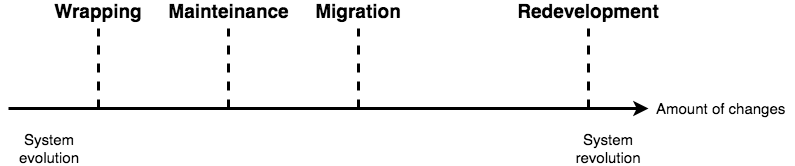
\includegraphics[width=.80\textwidth]{coping-with-legacy-systems}
\caption{Four approaches to cope with legacy software systems~\cite{bisbal-legacy-issues}}
\label{fig:coping-legacy}
\end{figure}


\subsubsection{Redevelopment}

To start from the far right, \textit{Redevelopment} is the most disruptive approach;
it implicates the discontinuation of the currently used software.
While having the huge disadvantage of being immensely cost-intensive, it indisputably
yields the best results opposed to the issues with legacy software presented in
subsection \ref{issues-legacy-software}.
Nevertheless, the second big risk apart from economic concerns is
the risk of failure.
Finally, depending on the size of the project, it is possible that at the end
of a long development cycle for the new software solution, it becomes outdated
yet again by not fully meeting the ever-changing
business needs anymore~\cite{stevens-software-reengineering-patterns}.


\subsubsection{Migration}

A median concept on the scale of figure \ref{fig:coping-legacy} is \textit{Migration}
which is also known as \textit{Reengineering}~\cite{tilley-perspectives-reengineering}.
These hypernyms actually describe two different solutions in terms of their goals;
they are, however, often used interchangeably~\cite{bisbal-legacy-issues}.
While both terms imply the extension of a legacy system, \textit{Reengineering}
has the goal to phase out the existing system eventually.
On the other hand, \textit{Migration} is just about augmenting the currently used
solution with new functional components while replacing some others that cannot be used anymore
for any reason. To put it into the words of Jesús Bisbal et al.:
\begin{displayquote}
\emph{"Migration seeks to reuse as much of the legacy information system as possible,
including implementation, design, specification, and requirements."}~\cite{bisbal-legacy-issues}
\end{displayquote}
Meanwhile, Scott R. Tilley and Dennis Smith define \textit{Reengineering} as:
\begin{displayquote}
\emph{"Reengineering is the systematic transformation of an existing system
into a new form […]"}~\cite{tilley-perspectives-reengineering}
\end{displayquote}
Consequently, these definitions put \textit{Reengineering} closer to \textit{Redevelopment},
due to the fact that both pursue the same long-term goal.
Nevertheless, \textit{Reengineering} is a type of \textit{Migration} and
therefore conducted similarly.\\
Concretely, there are four major approaches to a \textit{Migration}
process~\cite{malinova-legacy-techniques, seacord-modernizing-legacy},
ranging from a moderate one to the just mentioned \textit{Reengineering}
which is oftentimes a larger proposition.

\paragraph{Retargeting}
If for any reason the hardware or utilized third-party software got outdated,
the legacy software can be migrated to more performant hardware or
up-to-date versions of the leveraged third-party software.\\
\textit{Example}: Migrating the existing legacy software from traditional server
hardware to cloud-computing.

\paragraph{Conversion}
However, the changes in hardware or third-party software might be too disruptive
to perform them directly. In that case, a \textit{Conversion} of utilized
programming languages or technology stacks can be conducted.
Of course, this process is accompanied by much more work.\\
\textit{Example}: Converting the existing non-relational database to a
new database management system (DBMS) which is based on the relational SQL.

\paragraph{COTS components}
Furthermore, \textit{commercial-off-the-shelf (COTS) components} can be
leveraged to replace certain parts of a legacy software which oftentimes also
augments it, owing to the fact that such products are usually offering a wide
variety of features.\\
\textit{Example}: Replacing the customer management component of an existing
legacy software with a current COTS \textit{customer relationship management (CRM)} solution.

\paragraph{Reengineering}
As already mentioned, this last approach is the most labor-intensive yet most promising one.
During this procedure, the codebase gets refactored or reengineered
into completely new components which then replace outdated ones.
However, this process happens over time opposed to a \textit{Redevelopment} approach.\\
\textit{Example}: Transfer an increasing amount of distinct components
of the legacy application into web services.


\subsubsection{Wrapping}

To conclude, \textit{Wrapping} is the least revolutionary process.
In fact, it actively endorses the continuation of a legacy software solution as
portrayed in subsection \ref{sub-sect:continue-legacy}.
This concept involves wrapping the existing codebase into an isolated package
which is then just accessed via a newly created interface e.g. an API.
The existing legacy software receives input parameters and returns an output.
The substantial problem with this whole concept is that the legacy software does get
extended only unidirectionally. It cannot invoke calls towards the newly added components.
Therefore, this solution is rather short-term in nature.
This concept can be divided into four disparate levels~\cite{sneed-encapsulating-legacy}.

\paragraph{Database}
A \textit{database wrapper} is the least interfering approach due to the fact that
the existing source code can stay as it is; it just exposes the database of the current system
to the outside.\\
\textit{Example}: The database table persisting the print jobs of an existing legacy software
is available for external programs.

\paragraph{Service}
The \textit{service wrapper} encapsulates distinct services from the legacy software
into callable entities which can thus be invoked from an external system.\\
\textit{Example}: The entire reservation system of an existing legacy software
can be called via an API by an external system.

\paragraph{Application}
An \textit{application wrapper} provides single classes or whole components for external usage.
It is similar to a \textit{service wrapper}, however, the wrapping is applied on a more
compartmentalized level.\\
\textit{Example}: The object of a class to create print jobs in a certain format
gets exposed to the outside, allowing it to be used by external programs.

\paragraph{Function}
Finally, \textit{function wrappers} attach to the most microscopic portions of a software ---
its functions. This approach can be useful if both low cohesion and low coupling are prevalent
in the present legacy software.\\
\textit{Example}: A single function that calculates a specific taxation value
can be invoked by an external process.
\newline

To sum up, Robert C. Seacord also mentions \textit{Black-Box Modernization} as well as
\textit{White-Box Modernization}~\cite{seacord-modernizing-legacy} which are
effectively \textit{Wrapping} and \textit{Migration}. To put this into words,
if an organization conducts the \textit{Wrapping} approach, the main goal is not
to handle the internals of the legacy software.
Meanwhile, a \textit{Migration} process embraces subtle changes to the codebase of the software.\\
In consequence, owing to the fact that most of the time \textit{Wrapping} still
involves some changes to the codebase, \textit{Migration} can be a better
approach since it results in a longer-term solution.\\
Nevertheless, the primary focus of both approaches is to achieve a greater
return on investment (ROI) compared to a \textit{Redevelopment}~\cite{tilley-perspectives-reengineering}.



\chapter{Analysis} \label{chap:analysis}

\epigraphhead[55]{\epigraph{Once a system becomes a ball of mud,
some developers find security and prestige in being the select few who
can understand and evolve it, while those who detest the mud […] run away.
The result is that the ball of mud is rarely cleaned up.}
{\textit{George H. Fairbanks}}}

This chapter is structured similarly to the \textit{\nameref{chap:fundamentals}}
chapter. The first part is about the system and software architecture of
a back-end application for the short-term rental of electric scooters.
Consequently, the stages of a software development process as depicted
in section \ref{sect:software-development-process} are being exhibited.
The second part discusses the legacy software solution by \textit{Kumpan}
in terms of its components, issues and solutions to these issues.


\section{Hypothetical software solution} \label{sect:hypothetical-solution}

\subsection{Requirements}

As stated in subsection \ref{subsect:requirements}, the first step of
requirements engineering is the \textit{Elicitation}.
For that purpose, three executive stakeholders
at \textit{Kumpan}, the corporate partner of this thesis, were interviewed
to obtain the requirements for an ideal back-end application for the
short-term rental of electric scooters.\\
The discussed hypothetical software solution is meant for being licensed to
the actual operators of such a rental business. Therefore, an operator
is expected to maintain the application. Additionally, according to the
mentioned \textit{Environments}, three first requirements emerge:

\paragraph{Organizational}
The operating organization will employ service workers who
control certain aspects of the software. They are therefore still users of the
software albeit not being the target group. At this point it is still unclear
how much personnel would be sufficient but a small team of service workers is
enough to execute the business process and to serve the paying users.

\paragraph{Operational}
The service workers will use the non-public front-end of the software within a
web browser. Therefore, the interfaces of the software should be usable by
a web-based front-end solution.

\paragraph{Business}
The whole business model will be based around paying users. Consequently,
a working automated billing process as well as arrears billing is absolutely
crucial. It is expected to leverage the services of a third-party payment
provider owing to the fact that the operating organizations do not want to
handle private credit card information and the likes.


\subsubsection{Use Case}

The interview with the stakeholders quickly resolved around the use case
of such an application which yielded many requirements:\\

The user will have to download a mobile application or use the web app
of the operating organization. Consequently, both types of front-end applications
should be able to use the back-end application.\\\\
No user should be able to do anything without being logged into their account.
Thus, an implemented enrollment process is mandatory.\\\\
Within that process the user will have to fill in his or her
contact information, a valid driver's license as well as billing information.\\\\
Finally, the customer has to accept the terms and conditions of the operating
organization as well as the chosen billing model as described in
section \ref{sect:electric-scooter-market}. The operator should be able to chose
their billing model for all the customers application-wide.\\\\
After successful enrollment, the user will be greeted with a map of the current
location. This map should display all the currently available scooters at
their respective locations. The user can then browse the selection
of scooters and eventually chose one to rent.\\\\
The rental process will begin with a reservation of the chosen scooter for
a arbitrary time that the operator should be able to change application-wide.\\\\
Consequently, during the reservation time and the actual rental period,
the scooter should not appear on the map anymore for other users.\\\\
Next, the user is granted the set timeframe to get to the chosen scooter.
If the user arrives to late, the scooter should re-appear on the map,
available to every customer.\\\\
Once he or she arrived, the scooter as well as its ignition can be remotely
unlocked by the press of a button inside of the mobile app.
The back-end application however actually sends the signal to the scooter to
unlock itself.\\\\
Afterwards, the user can begin the ride for a previously chosen timeframe
or even indefinitely. After being finished, the user can discard of the scooter
anywhere within a certain range set by the operator.\\\\
The operator also needs to see a map with every scooter regardless of battery
charge or availability, mainly to plan out the relocation of certain ones.\\\\
Finally, the scooter is getting locked again and will re-appear on the map for the other users.\\\\
Moreover, during the ride, the scooter constantly sends its location as well
as other information about the current speed and battery statistics.
These information will be sent to a separate server which just persists them
without processing them any further.
Consequently, the back-end application will regularly fetch the information data
from said external server to monitor every ongoing ride of all the customers.\\\\
If a user drives out of the allowed operating range, a notification will be sent
to the scooter of that user.\\\\
If the battery gets low on charge, the user will be warned as well to finish the ride.\\\\
Additionally, after said ride has ended the scooter should also not re-appear
on the map of available ones.\\\\
The threshold for the low battery condition should also be changeable
application-wide by the operator.\\\\
Finally, the billing process should begin after the ride.\\\\
Furthermore, the user should be able to get statistics about his or her rides
e.g. the driven distance, the costs, the average speed and theoretically
many more. Therefore, the back-end application should allow those information
to be accessed by each customer while not exposing the statistics of others.\\

These are all of the functional requirements;
Figure \ref{fig:use-case-diagram} is used to put them into perspective.\\

\begin{figure}[htbp]
\centering
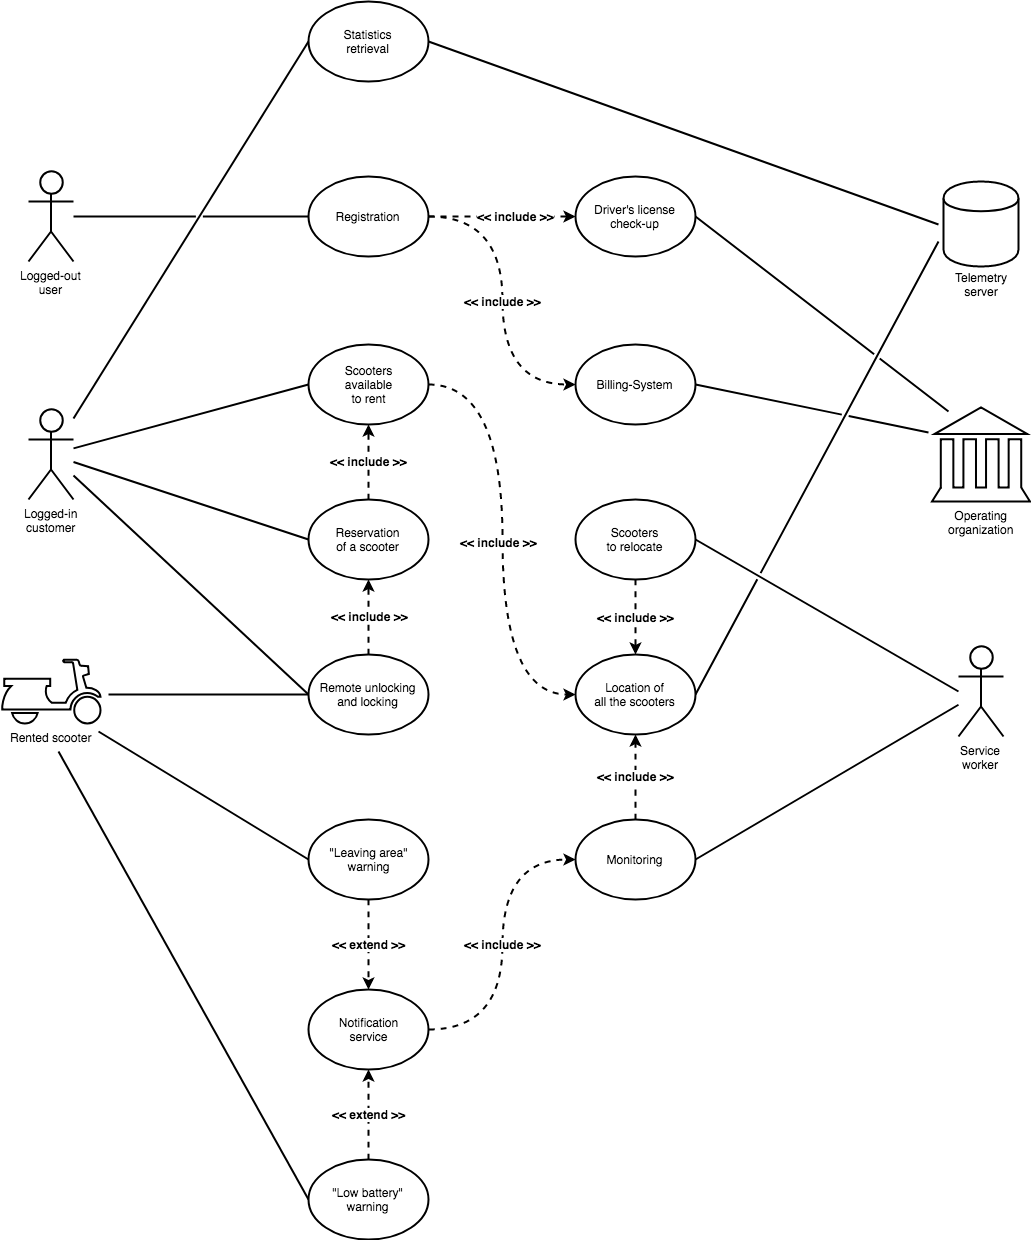
\includegraphics[width=1\textwidth]{use-case-diagram}
\caption{UML use case diagram based on the requirements of the hypothetical software solution}
\label{fig:use-case-diagram}
\end{figure}

Additionally, there is just one non-functional requirement.
As depicted in section \ref{sect:electric-scooter-market}, the current market
for the short-term rental of electric scooters is still fairly small.
Consequently, it is difficult to estimate how many users will use the system
in future years. Thus, the only non-functional requirement is that the system
should be easily scalable in case of a significant influx of new customers.


\subsection{Design}

The fundamentals of the software design are determined by answering the four
\textit{design decisions} posed in subsection \ref{subsect:design}.

\paragraph{What architectural patterns or styles might be used?}
A layered, monolithic approach poses the problem that it is too difficult
to integrate into an existing solution. In the end the old and the new
application would feasibly just communicate via API calls which would result
in two completely separate solutions. Furthermore, it is tedious to discern
which tasks get fulfilled by the old solution and which ones by the new one.
As a result, a vast interface in front of them both would be needed;
however that is an undesirable state for any application.

The system could follow an event-driven approach owing to the fact that
many of the depicted components of the use case have to run constantly without
much user interaction. Thus, implicitly invoked actions within the application
are feasible. Especially the \textit{Monitoring} component could benefit from
just publishing events while other components subscribe to them.
However, since an event-driven approach would require all the
functional components to work with events, the changes to the legacy solution
would be vast. For instance, while letting legacy components publish events
is still feasible, refactoring every possible interface to be able
to subscribe to events involves tremendous refactoring activities.

In contrast, the system could be structured in a service-oriented matter with
every larger component being a separate one. Other ones can be combined into
one service; however such decisions have to be made much more fine-grained.
The main advantage of the such an approach would be that it is easier to
integrate into an existing system compared to the other two approaches.
The modernization and extension of the legacy solution can be started with
re-developing a small component of the existing solution as a service.
Afterwards, the new service can be integrated into the legacy solution
in place of the old component.

In consequence, a service-oriented approach would best fit the depicted use case
while offering the possibility to iteratively extend and replace portions of
an existing legacy software solution with newly developed services.

\paragraph{What architectural organization is best for delivering the non-functional requirements of the system?}
Scaling is especially easy with a service-oriented approach. The single services
can be scaled up and down individually instead of scaling the whole application.
Some services will probably never see much load as they are not correlating with
increasing user counts whereas other services perform computation-intensive
actions as the monitoring of the scooter fleet; with a service-oriented approach,
the services in high demand can be scaled and even duplicated while others
remain as a single instance.

\paragraph{What will be the fundamental approach used to structure the system?}
A service-oriented approach already dictates the way an application is structured.
Each distinct group of tasks should be modeled into a separate service.
Even components that fulfill just a small task should exist as distinct services.
In summary, the functional requirements, and especially the components of
the use case diagram, should be separated into services based on their tasks.

\paragraph{What strategy will be used to control the operation of the components in the system?}
As stated in subsection \ref{subsect:design}, a service-oriented approach
requires much more middleware than e.g. a layered architecture.
The single services will be controlled and orchestrated via the middleware components
exhibited in the subsection on \textit{\nameref{subsubsect:architectural-styles}}.


\subsubsection{Architecture}

To model the software architecture, all of the components are getting divided
into distinct services based on their tasks. Consequently, many of the
\textit{Principles} stated in subsection \ref{subsect:design} are already fulfilled
partially or even completely. Good \textit{Decomposition and Modularization} is
easy to achieve in a service-oriented architecture --- the single services
are a direct application of \textit{Decomposition}.
Moreover, \textit{Information Hiding} is also a given fact when using a
service-oriented architecture.
Additionally, owing to the fact that a separate front-end will utilize the API
of the back-end, the interface and the implementation will be completely separated.
This statement is even corroborated by the fact that there will be three front-ends,
a mobile app as well as a web-based one for the customers additionally to the
web-based front-end for the service workers of the operating organization.
Finally, the shown services are modeled to feature a maximum of \textit{Abstraction}
as well as low \textit{Coupling}. This is achieved by splitting up components
into smaller services, should their tasks be too fine-grained without being
bound too much to them.

Based on these assumptions and the answered \textit{design decisions},
a diagram is utilized to portray the software architecture of the
\textit{Hypothetical software solution} as figure \ref{fig:service-architecture}.\\

\begin{figure}[htbp]
\centering
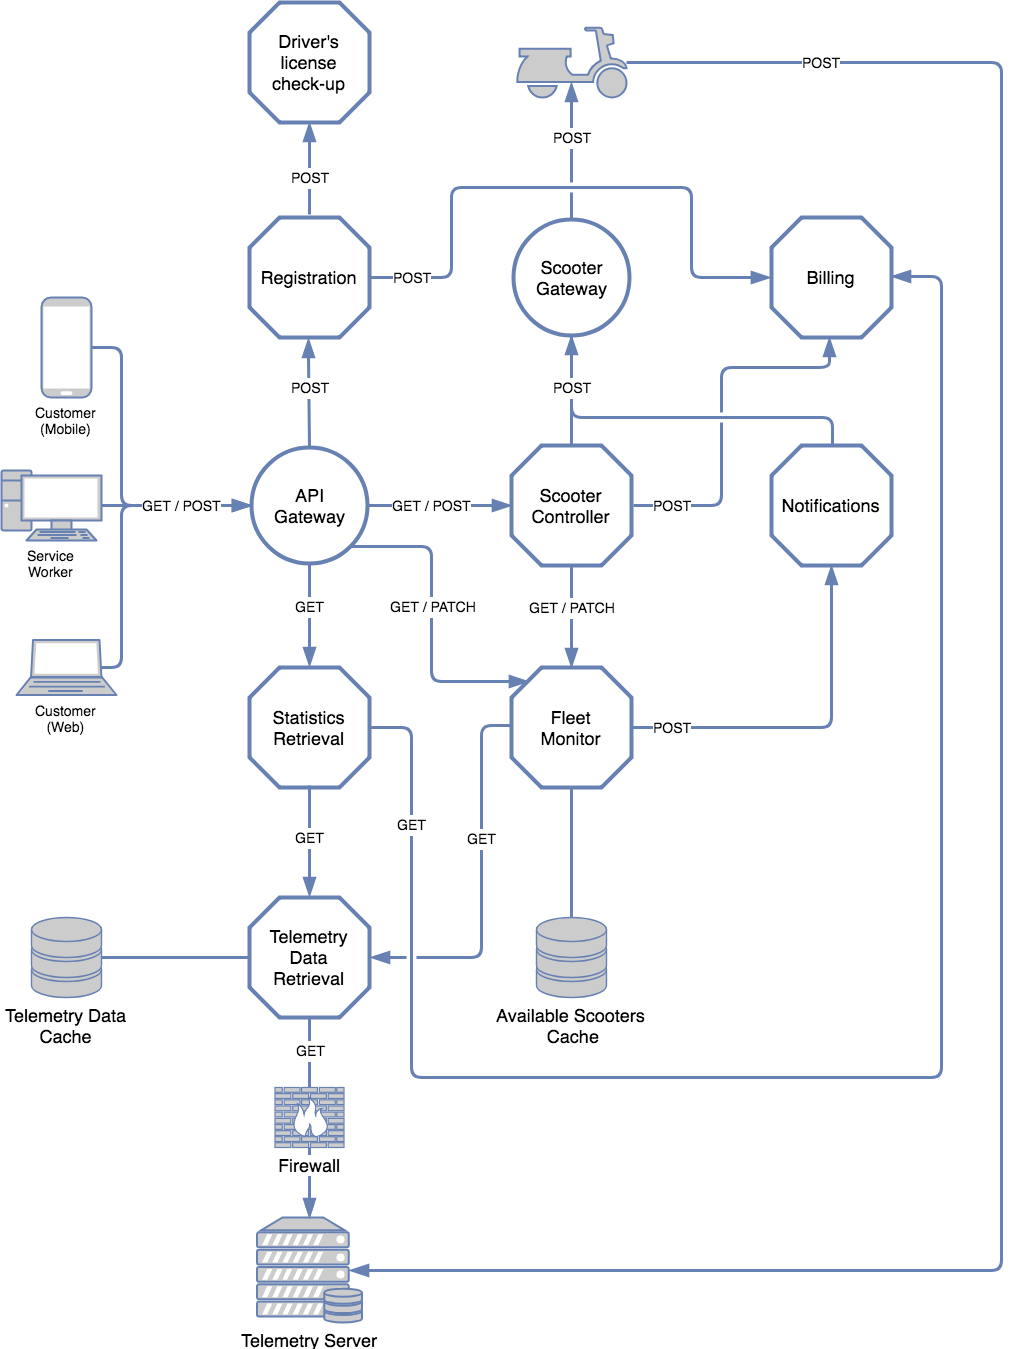
\includegraphics[width=1\textwidth]{service-architecture}
\caption{The hypothetical services and their intercommunication}
\label{fig:service-architecture}
\end{figure}

The diagram depicts the single services of the designed software architecture.
The arrows in between them denote the directions of HTTP requests as well
as the allowed HTTP methods for each request.
This can be an important indicator to conceive which services
will only be hit by \textit{GET requests} which are by definition \textit{safe},
in the way that they will never mutate any data~\cite{http-rfc}.
For example, the \textit{Telemetry Data Retrieval} service will never modify
its underlying data upon requests from other services.

All the services in the diagram are equipped with a RESTful API.
Each of them implements their own API that provides the functionalities that
should be available for the other services.

The \textit{API Gateway} has two tasks in this architecture.
Firstly, it serves as a literal gateway to shield all the services from
the outside and especially from the HTTP requests of the users.
This is mainly a security measurement so the services do not have to
implement authorization each on their own. Instead, the \textit{API Gateway}
checks that every user is authenticated and authorized to access certain
API endpoints. Thus, the services just accept API calls coming directly from
the \textit{API Gateway} to ensure that they have been verified to be eligible
for further handling.\\
Secondly, it provides the API endpoints that are actually available from the
outside as each service has their own host address and port number.
Thus, without the \textit{API Gateway} these information would need to be
directly exposed towards the front-end applications. Moreover, with cloud-based
deployments they might change in the future which would make the information
outdated on the client side.

Similarly, the \textit{Scooter Gateway} fulfills the same task towards the
fleet of scooters. The other services can just pass the
information they want to dispatch to a certain scooter to the
\textit{Scooter Gateway} which then sends the actual request to the scooter.
In this way, the services do not need to hold information on the host addresses
and port numbers of each scooter which makes the handling of them through
a shared gateway tremendously easier. Otherwise, the information would need
to exist redundantly as well since currently two different services are
dispatching requests towards scooters.

As already portrayed in the use case diagram (figure \ref{fig:use-case-diagram}),
the users of the back-end application will consist of service workers employed
by the operating organization as well as the customers.
The authorization towards the \textit{API Gateway} will determine which
API endpoints customers can access and which ones are just available to
service workers. For instance, the locations and information of all the scooters
of the fleet will just be available to authorized service workers via the
\textit{Fleet Monitor} service.

The \textit{Telemetry Data Retrieval} service fetches current data from the
off-site \textit{Telemetry Server} in periodical intervals.
Consequently, there will be a firewall in between these components.
This data consists of information such as the locations of all the scooters
of the fleet, their remaining battery power, as well as other information.
These information are crucial for the whole application.
Every scooter sends said information to the \textit{Telemetry Server}
periodically as well.

There should be two caches in the architecture to take away load from the
adjacent services. First, the aforementioned \textit{Telemetry Data Retrieval}
service will save new data into the cache which will automatically clear old
data after a preset amount of time. Thereby, nearly all of the requests from
other services apart from the \textit{Statistics Retrieval} one will hit the
\textit{Telemetry Data Cache} as those are only working with current data due
to their monitoring nature.\\
Second, the \textit{Available Scooter Cache} exists which provides the locations
of all the currently available scooters to customers that are currently looking
for a scooter to rent. Owing to the fact that this data will be requested by
many users very often, a cache is a good way to take away that potential load
from the \textit{Fleet Monitor} service which is already the one with
presumably the heaviest load.

The \textit{Driver's license check-up} as well as the \textit{Billing} service
will be closely related to third-party providers of such tasks.\\

Additionally to the use case diagram, a swimlane diagram
(figure \ref{fig:swimlane-rental-process}) has been created to depict
the flow of information between the customer, the scooter and the
involved services during the process of successfully renting a scooter.
This use case is by far the most important one which distinguishes oneself
from other common use cases e.g. registering an account.

\begin{figure}[htbp]
\centering
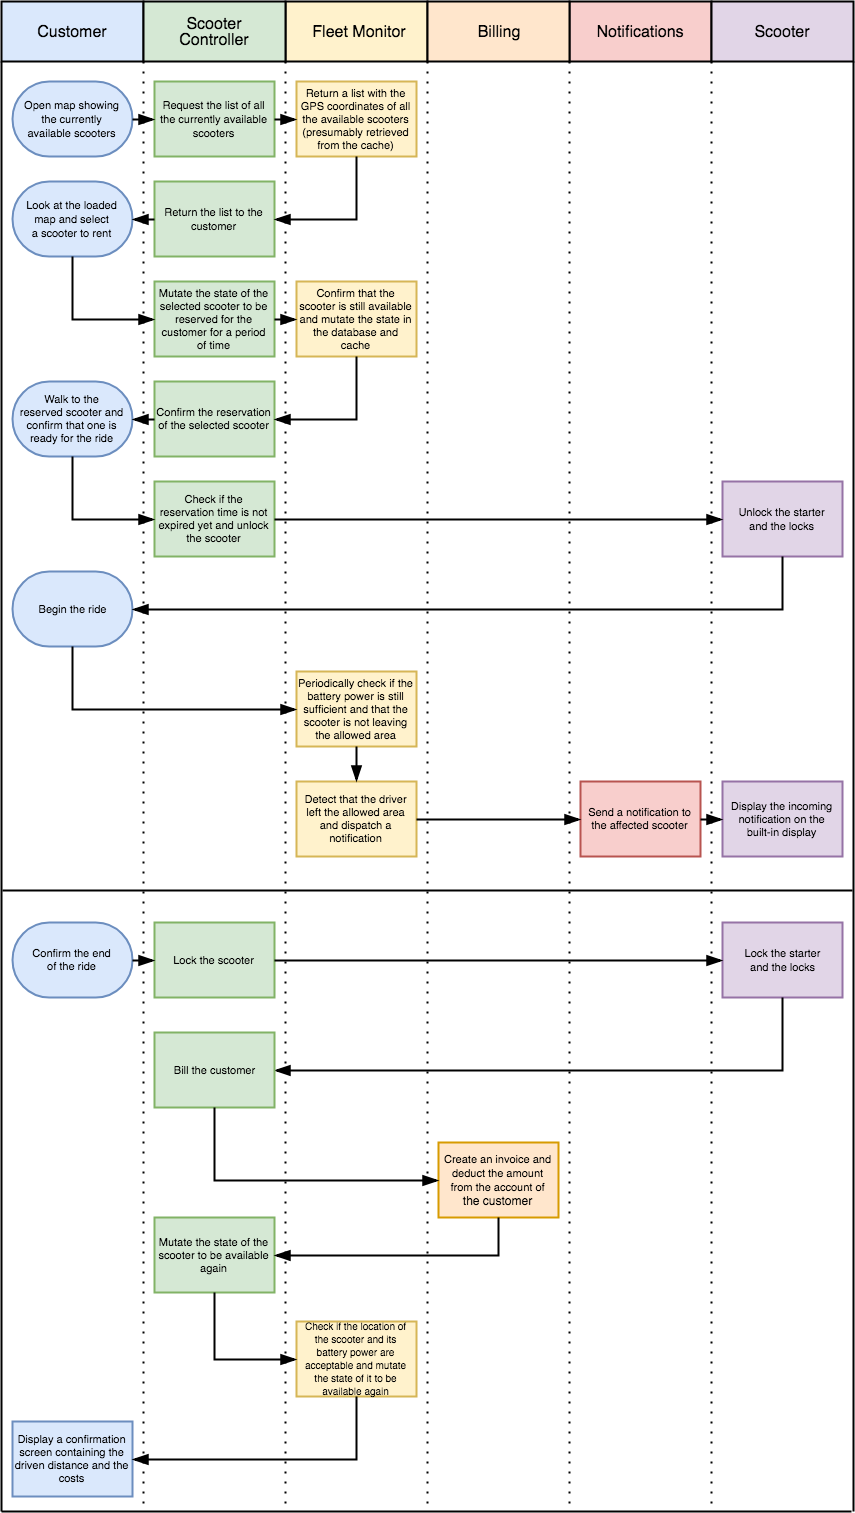
\includegraphics[width=1\textwidth]{swimlane-rental-process}
\caption{Swimlane diagram portraying the rental process}
\label{fig:swimlane-rental-process}
\end{figure}

The oval shapes represent user interactions whereas the square shapes represent
machine actions.

The solid horizontal line in the middle depicts the customer riding the scooter
which can take an indeterminate amount of time while no information is flowing.


\subsection{Construction}



\section{Legacy software solution} \label{sect:legacy-solution}

\subsection{Structure}

Structure


\subsection{Issues}

Issues


\subsection{Possible solutions}

Possible solutions


\chapter{Implementation} \label{chap:implementation}




\chapter{Conclusion} \label{chap:conclusion}




\newpage

% Source lists
\listoffigures
% \listoftables
\newpage

% Separate the sources with 'bibtopic'
\bibliographystyle{plain}
\begin{btSect}{references}
\section*{References}
\btPrintCited
\end{btSect}
\begin{btSect}{online}
\section*{Online Sources}
\btPrintCited
\end{btSect}

\end{document}
